\section{R3: Fabric Profiling for Rack-scale Architectures}
\label{sec:fabricprofile}

\begin{figure}[!t]
  \centering
  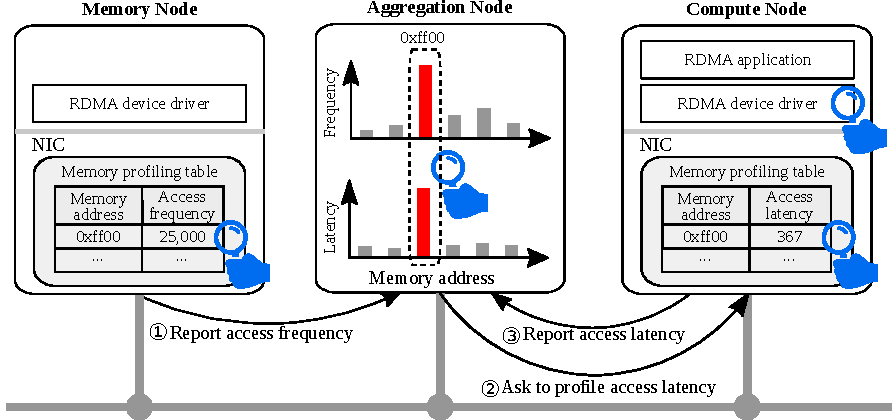
\includegraphics[width=0.8\textwidth]{fig/fabric-prof}
  \caption{
    Overview of the fabric profiler. Each memory node periodically
    reports hot memory locations with their access frequencies to an
    aggregation node \protect\C{1}. The aggregation node asks
    profiling of memory access latencies of the frequently accessed
    locations to compute nodes \protect\C{2}. Then, each compute node
    periodically reports access latencies of the chosen hot locations
    to the aggregation node \protect\C{3}. To minimize the performance
    overhead, we will take a hardware/software co-profiling approach;
    memory access frequency and latency are measured by an
    FPGA-implemented performance monitoring unit on a NIC;
    for hotspots, code paths will be associated using software
    profiling at the RDMA device driver.
  }
\label{f:fabric-overview}
\vspace{-5px}
\end{figure}

Fast interconnect fabrics (e.g., InfiniBand, RoCE,
Omni-Path~\cite{omnipath:web}, and GenZ~\cite{genz:web})
provide extremely high bandwidth (e.g.,
200Gbps~\cite{mellanox:200gb:web}) and low latency (e.g., 600
nanoseconds~\cite{mellanox:200gb:web}).
%
The low latency enables the exploration of a new level of hardware resource
sharing, so-called rack-scale architecture or disaggregated rack. Thus, the
disaggregation of hardware resources (e.g., memory, CPU, and NVMe) either at
the rack level or at the datacenter level is the direction for next-generation
data centers~\cite{sangjin:disaggregation, peter:disaggregation,
  ana:flash, rackintel:web, facebook:rackscale:web,
  oracle:sonoma:web}.
%
Remote direct memory access (RDMA) is the de-facto standard software
interface to use fabric interconnects. RDMA is designed to minimize
CPU intervention to achieve high performance. For example, remote
memory can be accessed without remote CPU intervention by using
one-sided RDMA operations. Emerging RDMA-based applications (e.g.,
distributed key-value stores~\cite{john:ramcloud, anuj:herd,
  alek:farm}, transaction processing~\cite{anuj:fasst, drtm:sosp15},
and disaggregated flash~\cite{ana:flash}) are designed to fully
utilize hardware resources within a fabric network.

However, fully exploiting the potential of fabric
networks is challenging. In particular, many RDMA-based applications
suffer from latency spikes induced from memory
hotspots~\cite{alek:farm, john:ramcloud, anuj:herd, stanko:rackout}.
These hotspots are created because some nodes have to handle more requests
than usual, which results in NICs becoming congested. Latency spikes, which
increase tail latency, affect the overall performance.
Therefore, it is necessary to pinpoint memory hotspots and the causes of
latency spikes to optimize RDMA-based applications. Unfortunately, no
proper solution has been developed yet.

\boxbeg
\begin{Challenge}
  Profiling memory access in a fast fabric network is essential to optimize
  RDMA-based applications. But it is very challenging
  for several reasons: high aggregated traffic, extremely low latency,
  large address space to monitor, no CPU intervention in one-sided
  operations, the necessity of fabric-wide monitoring, and the lack of
  hardware performance monitoring unit at NIC. In particular,
  profiling overhead should be low enough to not affect normal
  operations so we can continuously profile memory bottlenecks like
  Google-wide profiling~\cite{gwp:micro10} to capture sporadic latency
  spikes.
\end{Challenge}
\boxend

In this research thrust, we will develop {\em fabric profiler}, whose
main goal is to identify memory hotspots in the rack-scale
architecture and quantify the latency spikes while accessing these
hotspots with low profiling overhead.
We will take a hardware-software co-profiling approach to
minimize profiling overhead. As shown in~\autoref{f:fabric-overview},
the fabric profiler comprises three parts: 1) a performance monitoring
unit (PMU) to measure the access frequency and latency at NIC,
2) a RDMA-Verbs profiler to associate the collected information from
the PMU to execution context, and 3) an aggregation node for
fabric-wide aggregation of profiling data. In particular, we will take
an approach of profiling at a NIC rather than at a fabric switch.
That is because the RDMA messaging layer has been
commonly adopted across different fabric networks and it is easier to
associate higher-level information (e.g., task id, call stack) at NIC
than at a fabric switch. We plan to implement PMU using FPGA to sample
memory access information at NIC without runtime overhead. We believe
using FPGA for PMU is a viable and practical solution for several
reasons: FPGAs are already built-in some
NICs~\cite{mellanox:prodcut:web}; they are already being deployed in the
datacenter~\cite{andrew:catapult, bojie:clicknp, amazon:f1:web};
we expect that they will be more ubiquitous because of a wider range of
FPGA solutions~\cite{intel:fpga}. Our fabric profiler will first find
memory hotspots by monitoring access frequency
(\autoref{sub:hotspot}); then it will monitor memory access latency for
identified hotspots and will associate memory accesses with their running
context (\autoref{sub:latency}). Finally, it will aggregate profiled
information in all nodes within a fabric network (\autoref{sub:agg}).

\subsection{R3.1 Monitoring Memory Hotspots}
\label{sub:hotspot}

\boxbeg
\begin{Challenge}
  To identify memory hotspots, we need to monitor all the relevant
  memory accesses without affecting the normal performance even in
  one-sided RDMA operations with no CPU intervention.
\end{Challenge}
\boxend

In a rack-scale architecture, NIC acts as a memory controller for the
RDMA operations. Thus, we will sample memory access at the NIC level by using our
PMU implemented with FPGA. The sampled memory access will be logged to
the memory profiling table to collect the access frequency of each
memory location. Then, the profiled memory access frequency will be reported to
the aggregation node periodically or when the table is about to
overflow. For frequently accessed memory locations (i.e., hotspots),
the aggregation node asks compute nodes to profile their access
latency to find latency spikes.

\subsection{R3.2 Monitoring Latency Spikes}
\label{sub:latency}

\boxbeg
\begin{Challenge}
  The challenge in monitoring latency spikes comes from the large
  volume of RDMA traffic across a large range of memory addresses to
  multiple nodes. In addition, monitoring overhead should be low enough to
  have no effect on normal operations. And execution context (e.g., task id,
  call stack) should be associated with latency spikes for developers.
\end{Challenge}
\boxend

To reduce monitoring overhead, we will profile latency only for the
identified hotspots in \autoref{sub:hotspot}. Since a NIC does not
provide the latency to a particular memory address, we will again
leverage the NIC PMU to measure the latency of a particular
location. When the latency is logged to the memory
profiling table, the RDMA-Verb profiler, which profiles at an RDMA device
driver level, associates a memory location with its execution
context. Profiled access latency will be reported to the aggregation
node periodically or when the table is about to overflow.

\subsection{R3.3 Aggregating Profiled Data}
\label{sub:agg}

\boxbeg
\begin{Challenge}
  To obtain the holistic view of the profiling information, the fabric
  profiler will aggregate the fine grain memory access latency
  information across all nodes. The challenge here is in accessing
  information from large number of endpoints with memory accesses to
  large address space. Depending on the number of nodes involved
  during the profiling, this aggregated information can be huge.
\end{Challenge}
\boxend

Our fabric profiler will refine this information by correlating the
latency spike with the data objects across the cluster. This
aggregated output will provide the developer with information such as
latency incurred to the same memory location from different
nodes. With this information, the application developer can reason
those data objects that are being accessed across multiple
nodes, and can correlate tail latency to remote memory operations. For
example, this will allow the existing applications, such as FaRM and
RAMCloud, to correlate the GET/PUT performance with the remote memory
read/write latency. Furthermore, it can also benefit systems like
Amazon Dynamo~\cite{amazon:dynamo} to gauge the latency spike on the
slowest reader/writer in the quorum, as they decide whether the
operation is complete after the read/write nodes have successfully
read or modified the contents.
